SHOCK contains various capabilities of the numerical method: 
\begin{enumerate}
\item fifth and ninth order WENO scheme (spatial discretization of first order derivatives)
\item sixth and tenth order centreal differences (spatial discretization of second order derivatives)
\item third and fourth order Runge-Kutta (temporal discretization)
\end{enumerate}
In the following the fifth order WENO scheme in combination with a tenth order central differences and fourth-order Runge-Kutta scheme is discussed in detail.

\subsection{WENO scheme}
The inviscid fluxes $F$, $G$ and $H$ are approximated by using a fifth order Weighted Essentially Non-Oscillatory (WENO) finite difference scheme corresponding to Jiang and Shu \cite{Jiang1996}.
Exemplary for the flux in $\xi$-direction, the fifth order scheme is explained in following.
The derivative of the flux $F$ at the mesh point $i$ is defined as
\begin{equation}
\left( \frac{\partial F}{\partial \xi} \right)_i =\frac{F_{i+ 1/2} -F_{i-1/2}}{\varDelta \xi}
\end{equation}
where the cell boundary fluxes $F_{i \pm \frac{1}{2}}$ are
\begin{eqnarray}
F_{i\pm \frac{1}{2}} & =& \sum_{m=0}^{r-1} \omega_m M^r_m
\\ \nonumber
M^r_m & =& \sum_{l=i+m-r+1}^{i+m} a^r_{m,l} F_{l}.
\label{eq:eq4}
\end{eqnarray}
$M^r_m$ is the $m-th$ of $r$ ($r=(N+1)/2=3$) sub-stencil with polynomial coefficients $a^r_{m,l}$ for $N=5-th$ order of approximation.
The normalized weighting coefficient $\omega_m$, defined as
\begin{eqnarray}
\label{eq:omega}
\omega_m &= \frac{\bar{\omega}_m}{\bar{\omega}_0+...+\bar{\omega}_{r-1}}
\\ \nonumber
\bar{\omega}_m &= \frac{b_m^r}{\left(\epsilon+IS_m\right)^2}
\end{eqnarray}
, preserves monotonicity in the vicinity of strong gradients by the means of the smoothness indicators $IS_m$.
The parameter $\epsilon$ is added to avoid a division by zero at smooth solutions and is set to $\epsilon \approx 10^{-150}$ which is close to the minimal floating point value.
The coefficients $b_m^r$ are called optimal coefficients for the $5-th$ order of accuracy in smooth solution regions.
\par
In order to improve the numerical stability of the scheme, the propagation direction of the characteristics is taken into account resulting in a decomposition of the flux into two parts
\begin{equation}
F_{i \pm 1/2}=F^{+}_{i \pm 1/2}+F^{-}_{i \pm 1/2}
\label{eq:lfs}
\end{equation}
where the algebraic sign of the eigenvalue $\lambda$ of the matrix $A=\partial F/ \partial U$ determines the propagation direction. 
Matrix $A$ can be transformed into the characteristic form $A=R\Lambda R^{-1}$ with the diagonal matrix of eigenvalues $\Lambda$, the right $R$ and the left eigenvector $R^{-1}$.
Due to the usage of the maximal eigenvalue $\lambda_{i,max}$ within the stencil, it is called a local Lax-Friedrichs flux-vector splitting.
Finally, inserting equation~\eqref{eq:lfs} into equation~\eqref{eq:eq4} for $i+1/2$ yields to
\begin{eqnarray}
F_{i+1/2}& =&\overbrace{\frac{1}{12}\left[ -F_{i-1}+7F_{i}+7F_{i+1}-F_{i+2} \right]}^{central\ term} + \nonumber \\
& &\sum_{c=1}^{5}\left[ -\Phi_N \left( 
R^{-1}_{s}\varDelta F^{s,+}_{i-3/2},
R^{-1}_{s} \varDelta F^{s,+}_{i-1/2},
R^{-1}_{s} \varDelta F^{s,+}_{i+1/2},
R^{-1}_{s} \varDelta F^{s,+}_{i+3/2}
\right) \right. \\
& &\left. +\Phi_N \left( 
R^{-1}_{s} \varDelta F^{s,-}_{i+5/2},
R^{-1}_{s} \varDelta F^{s,-}_{i+3/2},
R^{-1}_{s} \varDelta F^{s,-}_{i+1/2,s},
R^{-1}_{s} \varDelta F^{s,-}_{i-1/2}
\right) \right] R_{s} \nonumber
\end{eqnarray}
\begin{equation}
\varDelta F^{s,\pm}_{i+1/2}=F^{s,\pm}_{i+1}-F^{s,\pm}_{i}
\end{equation}
\begin{equation}
F^{s,\pm}_{i}=\frac{1}{2}\left(F^s_{i} \pm \lambda_{i,max} \hat{U}^s_{i} \right)
\end{equation}
where the function $\Phi_N$ computes the non-linear corrections added to the central term depending on the weighting coefficients shown in equation~\eqref{eq:omega}, the $s-th$ component of the flux differences $\varDelta F^{\pm,c}_{i+1/2}$ and the eigenvectors $R^c$ and $R^{-1,c}$.
\begin{figure}[!ht]
  \begin{center} 
    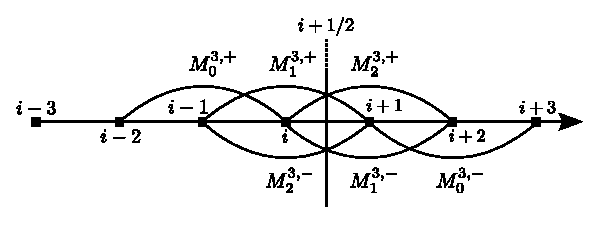
\includegraphics[width=0.5\linewidth]{stencil_weno5}
  \end{center}
  \caption {Schematic illustration of flux calculation for the cell boundary flux $F_{i + 1/2}$}
  \label{fig:fluxcalculation}
\end{figure}
Figure~\ref{fig:fluxcalculation} demonstrates the sub-stencil configuration for the whole flux calculation including the Lax-Friedrichs flux-vector splitting.

\subsection{Central differences scheme}
The viscous fluxes $F^\nu$, $G^\nu$ and $H^\nu$ are approximated by using a tenth order central-difference scheme. 
The approximation of the derivation is computed corresponding to the Taylor series.
\subsubsection{Double derivation: $\frac{\partial^2}{\partial \xi^2}$}
\begin{equation}
\left. \frac{\partial^2 u}{\partial \xi^2}\right|_{i,j}=\frac{A_{i+\frac{1}{2},j} \left(\frac{\partial u}{\partial \xi}\right)_{i+\frac{1}{2},j}-A_{i-\frac{1}{2},j} \left(\frac{\partial u}{\partial \xi}\right)_{i-\frac{1}{2},j}}{\varDelta \xi}
+\mathcal O\left(\varDelta \xi^{10}\right)
\end{equation}
with:
\begin{eqnarray}
\left(A \frac{\partial u}{\partial \xi}\right)_{i+\frac{1}{2},j}&=
C_{D,0}\left(u_{i+1}-u_{i} \right)\\ \nonumber
&-C_{D,1}\left(u_{i+2}-u_{i-1} \right)\\ \nonumber
&+C_{D,2}\left(u_{i+3}-u_{i-2} \right)\\ \nonumber
&-C_{D,3}\left(u_{i+4}-u_{i-3} \right)\\ \nonumber
&+C_{D,4}\left(u_{i+5}-u_{i-4} \right)
\\
\left(\frac{\partial u}{\partial \xi}\right)_{i-\frac{1}{2},j}&=
C_{D,0}\left(u_{i}-u_{i-1} \right)\\ \nonumber
&-C_{D,1}\left(u_{i+1}-u_{i-2} \right)\\ \nonumber
&+C_{D,2}\left(u_{i+2}-u_{i-3} \right)\\ \nonumber
&-C_{D,3}\left(u_{i+3}-u_{i-4} \right)\\ \nonumber
&+C_{D,4}\left(u_{i+4}-u_{i-5} \right)
\end{eqnarray}
\begin{equation}
C_{D,0}=-\frac{3}{9450}\ \ 
C_{D,1}=\frac{351}{75600}\ \ 
C_{D,2}=-\frac{2649}{75600}\ \ 
C_{D,3}=\frac{15351}{75600}\ \ 
C_{D,4}=-\frac{110649}{75600}
\end{equation}

\subsubsection{Mixed derivation: $\frac{\partial}{\partial \xi} \left(A\frac{\partial u}{ \partial \eta}\right)$}
\begin{equation}
\frac{\partial}{\partial \xi} \left(A\frac{\partial u}{ \partial \eta}\right)=
\frac{ \left. A\frac{\partial u}{\partial \eta}\right|_{i+\frac{1}{2},j} - \left. A\frac{\partial u}{\partial \eta}\right|_{i-\frac{1}{2},j}}{\varDelta \xi}
+\mathcal O\left(\varDelta \xi^{10}+\varDelta \eta^{10}\right)
\end{equation}

with interpolation coefficients:
\begin{eqnarray}
\left. A\frac{\partial u}{\partial \eta}\right|_{i+\frac{1}{2},j}&=
C_{P,0}\left(\left. A\frac{\partial u}{\partial \eta}\right|_{i+1,j}+\left. A\frac{\partial u}{\partial \eta}\right|_{i,j} \right)\\ \nonumber
&-C_{P,1}\left(\left. A\frac{\partial u}{\partial \eta}\right|_{i+2,j}+\left. A\frac{\partial u}{\partial \eta}\right|_{i-1,j} \right)\\ \nonumber
&+C_{P,2}\left(\left. A\frac{\partial u}{\partial \eta}\right|_{i+3,j}+\left. A\frac{\partial u}{\partial \eta}\right|_{i-2,j} \right)\\ \nonumber
&-C_{P,3}\left(\left. A\frac{\partial u}{\partial \eta}\right|_{i+4,j}+\left. A\frac{\partial u}{\partial \eta}\right|_{i-3,j} \right)\\ \nonumber
&+C_{P,4}\left(\left. A\frac{\partial u}{\partial \eta}\right|_{i+5,j}+\left. A\frac{\partial u}{\partial \eta}\right|_{i-4,j} \right)
\\
\left. A\frac{\partial u}{\partial \eta}\right|_{i-\frac{1}{2},j}&=
C_{P,0}\left(\left. A\frac{\partial u}{\partial \eta}\right|_{i,j}+\left. A\frac{\partial u}{\partial \eta}\right|_{i-1,j} \right)\\ \nonumber
&-C_{P,1}\left(\left. A\frac{\partial u}{\partial \eta}\right|_{i+1,j}+\left. A\frac{\partial u}{\partial \eta}\right|_{i-2,j} \right)\\ \nonumber
&+C_{P,2}\left(\left. A\frac{\partial u}{\partial \eta}\right|_{i+2,j}+\left. A\frac{\partial u}{\partial \eta}\right|_{i-3,j} \right)\\ \nonumber
&-C_{P,3}\left(\left. A\frac{\partial u}{\partial \eta}\right|_{i+3,j}+\left. A\frac{\partial u}{\partial \eta}\right|_{i-4,j} \right)\\ \nonumber
&+C_{P,4}\left(\left. A\frac{\partial u}{\partial \eta}\right|_{i+4,j}+\left. A\frac{\partial u}{\partial \eta}\right|_{i-5,j} \right)
\end{eqnarray}

The derivations are computed by:

\begin{equation}
\left. \frac{\partial u}{\partial \eta}\right|_{i,j}=\frac{u_{i,j+\frac{1}{2}}-u_{i,j-\frac{1}{2}}}{\varDelta \eta}\\
\end{equation}

with:

\begin{eqnarray}
u_{i,j+\frac{1}{2}}&=
C_{P,0}\left(u_{i,j+1}+u_{i,j} \right)\\ \nonumber
&-C_{P,1}\left(u_{i,j+2}+u_{i,j-1} \right)\\ \nonumber
&+C_{P,2}\left(u_{i,j+3}+u_{i,j-2} \right)\\ \nonumber
&-C_{P,3}\left(u_{i,j+4}+u_{i,j-3} \right)\\ \nonumber
&+C_{P,4}\left(u_{i,j+5}+u_{i,j-4} \right)
\\
u_{i,j-\frac{1}{2}}&=
C_{P,0}\left(u_{i,j}+u_{i,j-1} \right)\\ \nonumber
&-C_{P,1}\left(u_{i,j+1}+u_{i,j-2} \right)\\ \nonumber
&+C_{P,2}\left(u_{i,j+2}+u_{i,j-3} \right)\\ \nonumber
&-C_{P,3}\left(u_{i,j+3}+u_{i,j-4} \right)\\ \nonumber
&+C_{P,4}\left(u_{i,j+4}+u_{i,j-5} \right)
\end{eqnarray}
\begin{equation}
C_{P,0}=\frac{1}{1260}\ \ 
C_{P,1}=-\frac{23}{2520}\ \ 
C_{P,2}=\frac{127}{2520}\ \ 
C_{P,3}=-\frac{473}{2520}\ \ 
C_{P,4}=\frac{1627}{2520}\\
\end{equation}

\subsection{Explicit Runge-Kutta scheme}
For time integration an explicit, fourth order, low storage, total variation diminishing (TVD) Runge-Kutta scheme is applied.
\begin{eqnarray}
U_{A}&=U^{n}+ \frac{\varDelta t}{2} Q\left(U^{n}\right)\\
U_{B}&=U_{A}+ \frac{\varDelta t}{2} \left(-Q\left(U^{n}\right)+Q\left(U_{A}\right)\right)\\
U_{C}&=U_{B}+ \frac{\varDelta t}{2} \left(-Q\left(U_{A}\right)+2Q\left(U_{B}\right)\right)\\
U^{n+1}&=U_{C}+\frac{\varDelta t}{6} \left(Q\left(U^{n}\right)+2Q\left(U_{A}\right)-4Q\left(U_{B}\right)+Q\left(U_{C}\right)\right)
\end{eqnarray}

yields to:

\begin{eqnarray}
U_{A}&= U^{n}+ \frac{\varDelta t}{2} Q\left(U^{n}\right)\\
U_{B}&=U^{n}+ \frac{\varDelta t}{2} Q\left(U_{A}\right)\\
U_{C}&=U^{n}+ \varDelta t\ Q\left(U_{B}\right)\\
U^{n+1}&=U^{n}+\frac{\varDelta t}{6}Q\left(U_{C}\right)+\frac{\varDelta t}{6} \underbrace{ \left[Q\left(U^{n}\right)+2 Q\left(U_{A}\right)+2 Q\left(U_{B}\right)\right]}_{Q_{sum}}
\end{eqnarray}